\documentclass[../main/main.tex]{subfiles}
\graphicspath{{./figures/}}
\usepackage{pdfpages}

\makeatletter
\renewcommand{\@chapapp}{Travaux pratiques -- TP}
\makeatother

% \toggletrue{student}
\HideSolutionstrue
\toggletrue{corrige}
% \renewcommand{\mycol}{black}
\renewcommand{\mycol}{gray}

\begin{document}
\setcounter{chapter}{13}

\chapter{\cswitch{Correction du TP}{\'Etude d'un filtre actif du second ordre}}

\enonce{
	\begin{prgm}
		\begin{tcb}*(ror)"how"{Savoir-faire}
			\begin{itemize}
				\item Mettre en œuvre un dispositif expérimental illustrant l’utilité
				      des fonctions de transfert pour un système linéaire à un ou plusieurs
				      étages.
				\item Utiliser une fonction de transfert donnée d’ordre 1 ou 2 (ou ses
				      représentations graphiques) pour étudier la réponse d’un système
				      linéaire à une excitation sinusoïdale
			\end{itemize}
		\end{tcb}
	\end{prgm}
	\vspace{-10pt}
	\section{Objectifs}
	\begin{itemize}
		\item Être attentif-ve aux problèmes liés aux masses des appareils de
		      mesure.
		\item Apprécier rapidement le comportement en fréquence d'un filtre par
		      balayage rapide avant de faire les mesures.
		\item Effectuer les mesures permettant de tracer le diagramme de Bode en
		      amplitude d'un filtre.
		\item Utiliser un multimètre en mode dBmètre.
		\item Apprendre à tracer un diagramme de Bode sur papier
		      semi-logarithmique~: fréquence de coupure à $-\SI{3}{dB}$, bande
		      passante, nature et ordre du filtre.
	\end{itemize}

	\section{Méthode pour mesurer un gain en dB (rappel)}

	\begin{tcb}(rapp)<itc>{Rappel~: mesure de gain}
		\begin{enumerate}
			\item Appuyez sur la fonction Volt alternatif (symbole
			      \fbox{V$\sim$}), \textbf{puis} dBmètre (bouton \fbox{dB}) pour
			      activer la fonction dBmètre~;
			\item Brancher le multimètre sur l'entrée $e(t)$ du montage~;
			\item Appuyer sur \fbox{\texttt{rel}} une ou deux fois jusqu'à ce que le
			      multimètre affiche 0~: on indique alors au multimètre que c'est cette
			      tension $e(t)$ qui sert de référence.
			\item Brancher ensuite le multimètre sur la sortie $s(t)$. Il affiche
			      directement le gain en dB.
		\end{enumerate}
	\end{tcb}

	\begin{tcb}[cnt,bld](impo){Attention~!}
		Il faut refaire le zéro relatif pour chaque fréquence.
	\end{tcb}
}

\setcounter{section}{2}
\section{Analyser}

\enonce{%
	\noindent
	\begin{minipage}{0.50\linewidth}
		Le filtre de \textsc{Rauch} est un filtre actif, c'est-à-dire qu'il est
		alimenté électriquement par un générateur extérieur pour fonctionner. Il
		repose sur l'utilisation de 5 dipôles passifs et d'un amplificateur
		opérationnel (AO). Ces derniers ne sont pas au programme de première année.
		Il n'est donc pas possible pour vous de déterminer la fonction de transfert
		associée à ce filtre. Vous pouvez donc voir le filtre comme une boîte noire
		qui réalise la fonction de transfert suivante~:
		\[
			\boxed{
				\Hu(\jj \w) = \frac{\su}{\eu} = \frac{H_0}{1+\jj Q
					\left(\dfrac{\w}{\w_0}-\dfrac{\w_0}{\w}\right)}
			}
		\]
	\end{minipage}
	\hfill
	\begin{minipage}{0.45\linewidth}
		\begin{center}
			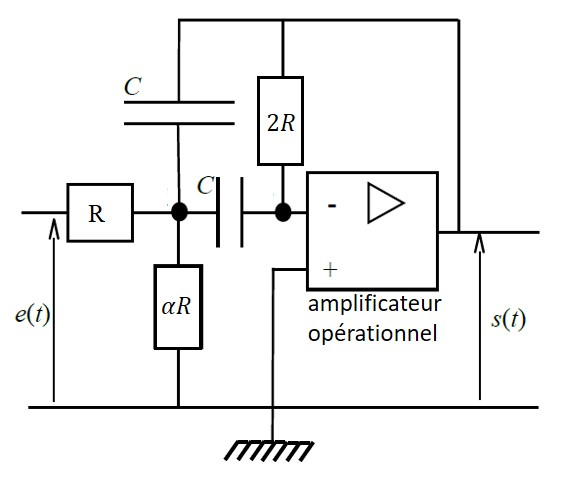
\includegraphics[width=\linewidth]{rauch_montage}
		\end{center}
	\end{minipage}

	\begin{gather*}
		\beforetext{Avec}
		Q = \sqrt{\frac{\alpha+1}{2\alpha}},
		\quad
		H_0 = -1
		\qet
		\w_0 = \sqrt{\frac{\alpha+1}{2\alpha}} \, \frac{1}{RC}
	\end{gather*}
	Ainsi, bien que ce filtre soit nouveau par rapport à ce que vous avez étudié, sa
	fonction de transfert est analogue à des cas étudiés en classe. Vous pouvez donc
	étudier sa fonction de transfert. Pour ce faire~:
}

\setlist[blocQR,1]{leftmargin=10pt, label=\clenumi}
\QR{%
	Déterminer les équations des asymptotes BF et HF du Bode en gain. En
	déduire la nature de ce filtre.
}{%
	On a ici $\abs{\Hu_0} = 1$, donc on peut réaliser la même étude qur le RLC sur
	R~:
	\begin{table}[htbp!]
		\centering
		\caption{Étude du filtre.}
		\begin{tabularx}{\linewidth}{cYYY}
			\toprule
			 &
			$\forall x$
			 &
			$x\to 0$
			 &
			$x\to\infty$
			\\
			\addlinespace[0.5em]
			\cmidrule(lr){2-4}
			$\DS\Hu = \frac{\Su}{\Eu}$
			 &
			$\DS \frac{1}{1+ \jj Q \left( x - \frac{1}{x} \right)}$
			 &
			$\DS \jj \frac{x}{Q}$
			 &
			$\DS -\jj \frac{1}{xQ}$
			\\
			\addlinespace[0.5em]
			$\DS G\ind{dB} = 20 \log \abs{\Hu}$
			 &
			$\DS -10 \log (1+Q^{2}\left( x - \frac{1}{x} \right)^{2})$
			 &
			$\DS 20 \log \left( \frac{x}{Q} \right)$
			 &
			$\DS -20 \log (Qx)$
			\\
			\bottomrule
		\end{tabularx}
		\label{tab:rlcr}
	\end{table}
	\smallbreak
	On trouvera également $G\ind{dB}(x=1) = 20 \log (\frac{\abs{\Hu_0}}{\sqrt{2}})
		= \SI{-3}{dB}$. Par l'étude des asymptotes, on obtient un passe-bande.
}
\QR{%
Déterminer la pulsation de résonance $\w_{r}$ en fonction de $\w_0$ et
$Q$. Déterminer la largeur de la bande passante de ce filtre en fonction
de $\w_0$ et $Q$, puis de $R$ et $C$.
}{%
On trouve le maximum de cette amplitude quand le dénominateur est minimal,
c'est-à-dire
\begin{gather*}
	H(\w_r) = H_{\max}
	\Lra
	1 + Q^2\left( \frac{\w_r}{\w_0} - \frac{\w_0}{\w_r} \right)^2 \text{minimal}\\
	\Lra
	Q^2\left( \frac{\w_r}{\w_0} - \frac{\w_0}{\w_r} \right)^2 = 0
	\Lra
	\boxed{\w_r = \w_0}
\end{gather*}
Et ainsi $H_{\max} = H_0$. Pour la bande passante, on commence par déterminer
les pulsations réduites $x_1$ et $x_2$ telles que $\abs{\Hu(x_i)} =
	\abs{H_0}/\sqrt{2}$~:
\begin{DispWithArrows*}
	1+Q^2 (x_i - 1/x_i)^2 &= 2
	\CArrow{$\sqrt{\cdot}$}
	\\\Lra
	Q \pa{x_i - \frac{1}{x_i}} &= \pm 1
	\Arrow{$\times x_i$}
	\\\Lra
	Q x_i{}^{2} \mp x_i - Q &= 0
	\Arrow{Discriminant}
	\\\Ra
	\Delta &= 1 + 4Q{}^{2}
	\Arrow{Solutions}
	\\\Ra
	x_{i,\pm,\pm} &= \frac{\pm 1 \pm \sqrt{1+4Q{}^{2}}}{2Q}
\end{DispWithArrows*}
On obtient alors deux polynômes du second degré (un avec le signe $+$, l'autre
avec le signe $-$). On ne garde que les racines positives, sachant que
$\sqrt{1+4Q{}^{2}} > 1$~:
\[
	x_1 = x_{i,-,+} = \frac{1}{2Q} \pa{-1 + \sqrt{1+4Q{}^{2}}}
	\qet
	x_2 = x_{i,+,+} = \frac{1}{2Q} \pa{1 + \sqrt{1+4Q{}^{2}}}
\]
puis on obtient
$x_2 - x_1 = 1/Q$ soit au final $\boxed{\Delta \w = \frac{\w_0}{Q} =
		\frac{1}{RC}}$.
}

\QR{%
	À quelle condition sur $\alpha$ ce filtre peut-il être efficace pour
	sélectionner individuellement les fréquences constituant le signal
	d'entrée~? On supposera, afin de fixer les idées, un signal d'entrée
	périodique (non sinusoïdal) de pulsation fondamentale $\w_{f}$ dont on
	souhaite sélectionner l'harmonique de rang 3 (pulsation $3\w_{f}$).
}{%
	Pour séletionner $3\w_f$, il faut que $\w_0 = 3\w_f$, mais aussi que le filtre
	soit \textbf{suffisamment fin} pour que les pulsations $2\w_f$ et $4\w_f$
	soient atténuées. En représentation spectrale, on obtient la figure suivante~:
	\smallbreak
	\noindent
	\begin{minipage}{.30\linewidth}
		On cherche donc à avoir~:
		\begin{DispWithArrows*}[fleqn, mathindent=2pt]
			\Delta\w &< \w_f
			\Arrow{$\w_f = \w_0/3$\\$\Delta\w = 1/RC$}
			\\\Lra
			\frac{1}{RC} &< \frac{1}{3}\w_0
			\Arrow{$\w_0 = \sqrt{\frac{\alpha+1}{2\alpha}} \, \frac{1}{RC}$}
			\\\Lra
			\cancel{\frac{1}{RC}} &< \frac{1}{3}
			\sqrt{\frac{\alpha+1}{2\alpha}}\cancel{\frac{1}{RC}}
			\Arrow{On isole}
			\\\Lra
			3^{2} &< \left( \sqrt{\frac{\alpha+1}{2\alpha}} \right)^{2}
			\Arrow{On simplifie}
			\\\Lra
			9 &< \frac{\alpha+1}{2\alpha}
			\Arrow[jump=2]{On isole}
			\\\Lra
			18\alpha &< \alpha+1
			\\\Lra
			\Aboxed{\alpha &< \frac{1}{17}}
		\end{DispWithArrows*}
	\end{minipage}
	\hfill
	\begin{minipage}{.50\linewidth}
		~
		\begin{center}
			\includegraphics[width=\linewidth]{selec_filtre}
		\end{center}
	\end{minipage}
  \smallbreak
	Il faut donc avoir $\alpha$ petit pour avoir $Q$ grand et sélectionner
	précisément des fréquences.
}

\QR{%
On prend $RC=\SI{1.0e-4}{s}$. Pour $\alpha= \num{e-2}$ puis $\alpha=1$,
préciser les coordonnées des points d'intersection des asymptotes BF et
HF $(f_{I}~;~G_{{\dB}, I})$.
}{%
Les asymptotes se croisent si
\vspace{-25pt}
\begin{DispWithArrows*}
	G\ind{dB}(x\to0) &= G\ind{dB}(x\to\infty)
	\Arrow{On remplace}
	\\\Lra
	20 \log (x) - \cancel{20 \log Q} &= -20 \log (x) - \cancel{20 \log Q}
	\Arrow{On simplifie}
	\\\Lra
	\log (x) &= 0
	\Arrow{On inverse le log}
	\\\Lra
  \Aboxed{x &= 1}
\end{DispWithArrows*}
\[
	\boxed{
		\left\{
		\begin{array}{rlcrl}
			f_{0,\alpha=\num{e-2}} & = \SI{11.4}{kHz}
			                       & \quad ;          & \quad
			G_{\dB,\num{e-2}}      & = \SI{-17}{dB}
			\\
			f_{0,\alpha=1}         & = \SI{1.6}{kHz}
			                       & \quad ;          & \quad
			G_{\dB,1}              & = \SI{0}{dB}
		\end{array}
		\right.
	}
\]
\vspace{-15pt}
\begin{tcb}(ror){Croisement asymptotes}
	En réalité, les asymptotes se croisent toujours en $x=1$ (mais il faut savoir
	le démontrer).
\end{tcb}
}
\section{Réaliser}

\enonce{%
  On étudie ce montage pour deux valeurs de $\alpha$. On prendra successivement
\[
  \boxed{\alpha=\num{e-2}} \qqMath{puis} \boxed{\alpha=1}
\]

Le filtre schématisé ci-dessus est une «~boite noire~» dans laquelle on trouve
un amplificateur opérationnel. Pour s'en servir, il faut au préalable polariser
l'amplificateur opérationnel, c'est-à-dire~:
\begin{tcb}(expe)<itc>{Manipulation amplificateur}
  \begin{enumerate}
    \item Connecter la borne \SI{+15}{V} du boitier à la sortie \SI{+15}{V} d'un
          générateur de tension continue,
    \item Connecter la borne \SI{-15}{V} du boitier à la sortie
          \SI{-15}{V} du générateur
    \item Connecter le point milieu du boitier à la masse du
          générateur.
          \begin{center}
            \begin{tcb}[cnt,bld,width=.9\linewidth](impo){Attention}
              À la fin de la séance, on coupe le signal du GBF avant les
              alimentations de l'amplificateur opérationnel qui doivent être
              coupées en dernier.
            \end{tcb}
          \end{center}
    \item Réalisez ensuite le montage en prenant $C=\SI{1}{nF}$ (cavalier prêt à
          être connecté sur la boite) et $\alpha R$ avec une boite de résistances
          variables.
  \end{enumerate}
\end{tcb}

On alimente le filtre avec un GBF en tension sinusoïdale et on souhaite
visualiser simultanément $e(t)$ sur la voie 1 et $s(t)$ sur la voie 2 de
l'oscilloscope. On utilisera le voltmètre pour mesurer le gain en dB.
}
\QR{%
	La «~boite noire~» a été fabriquée avec $R= \SI{100}{k\Omega}$.
	Déterminer la valeur à donner à $\alpha R$ pour $\alpha=\num{e-2}$.
}{%
  \centers{$\boxed{\alpha R = \SI{1}{k\Omega}}$}
  \vspace{-15pt}
}

\resetQ
\setlist[blocQR,1]{leftmargin=10pt, label=\sqenumi}
\QR{%
	\underline{Étude rapide}~: Faire varier la fréquence du signal d'entrée et
	vérifier rapidement que le filtre fonctionne correctement. En particulier,
	vous déterminerez la fréquence de résonance.
}{%
	On observe $f_{0,\exp} = \SI{11.30\pm0.01}{kHz}$ avec $\alpha=\num{e-2}$. On a
	bien une amplitude de sortie nulle pour les basses \textbf{et}  hautes
	fréquences~: c'est bien un passe-bande.
}
\QR{%
	\xul{Étude complète}~: Prendre comme amplitude du signal d'entrée $E_{m}
		\approx \SI{2}{V}$ puis, pour des fréquences entre $\SI{100}{Hz}$ et
	$\SI{80}{kHz}$, mesurer le gain en dB. Faire un tableau \textit{numérique}
	avec l'outil de votre choix (LatisPro recommandé, calculatrice recommandée) et
	imprimez ou réécrire les valeurs sur votre copie.
}{%
	Non corrigé.
}

\QR{%
	Recommencer les deux mêmes études pour $\alpha=1$.
}{%
	On observe $f_{0,\exp} = \SI{1.5\pm 0.1}{kHz}$ avec $\alpha=1$.
}

\section{Valider}

\QR{%
	Tracer, pour chacune des deux valeurs de $\alpha$, les diagrammes de
	Bode en gain expérimentaux sur papier semi-log en mettant la fréquence
	en abscisse. Ajouter sur ces deux diagrammes, les asymptotes obtenues
	grâce à l'étude théorique de l'analyse.
}{%
	Voir pages finales.
}

\section{Conclure}

\QR{%
	Quelle différence essentielle constate-t-on entre ces deux filtres~?
	Comment faire varier la capacité $C$ afin de faire varier $Q$ sans faire
	varier $\w_0$~?
}{%
	Les fréquences de résonance sont différentes, et la forme de la courbe varie~:
	la bande passent est la même, $\Delta\w = \frac{1}{RC}$, mais avec l'échelle
	log le diagramme avec $\alpha = \num{e-2}$ semble plus piquée.
	\smallbreak
	Pour changer $Q$ sans changer $\w_0$, il faut faire varier $C$ dans le même
	sens que $Q$~:
	\[
		\w_0 = \frac{Q}{RC}
		\quad ; \quad
		\w_0 = \cte
		\Ra
		\left\{
		\begin{array}{lcr}
			Q\nearrow & \text{et} & C\nearrow
			\\
			Q\searrow & \text{et} & C\searrow
		\end{array}
		\right.
	\]
}

\newpage
\enonce{%
  ~
\newpage
}

\thispagestyle{empty}
\cswitch{
	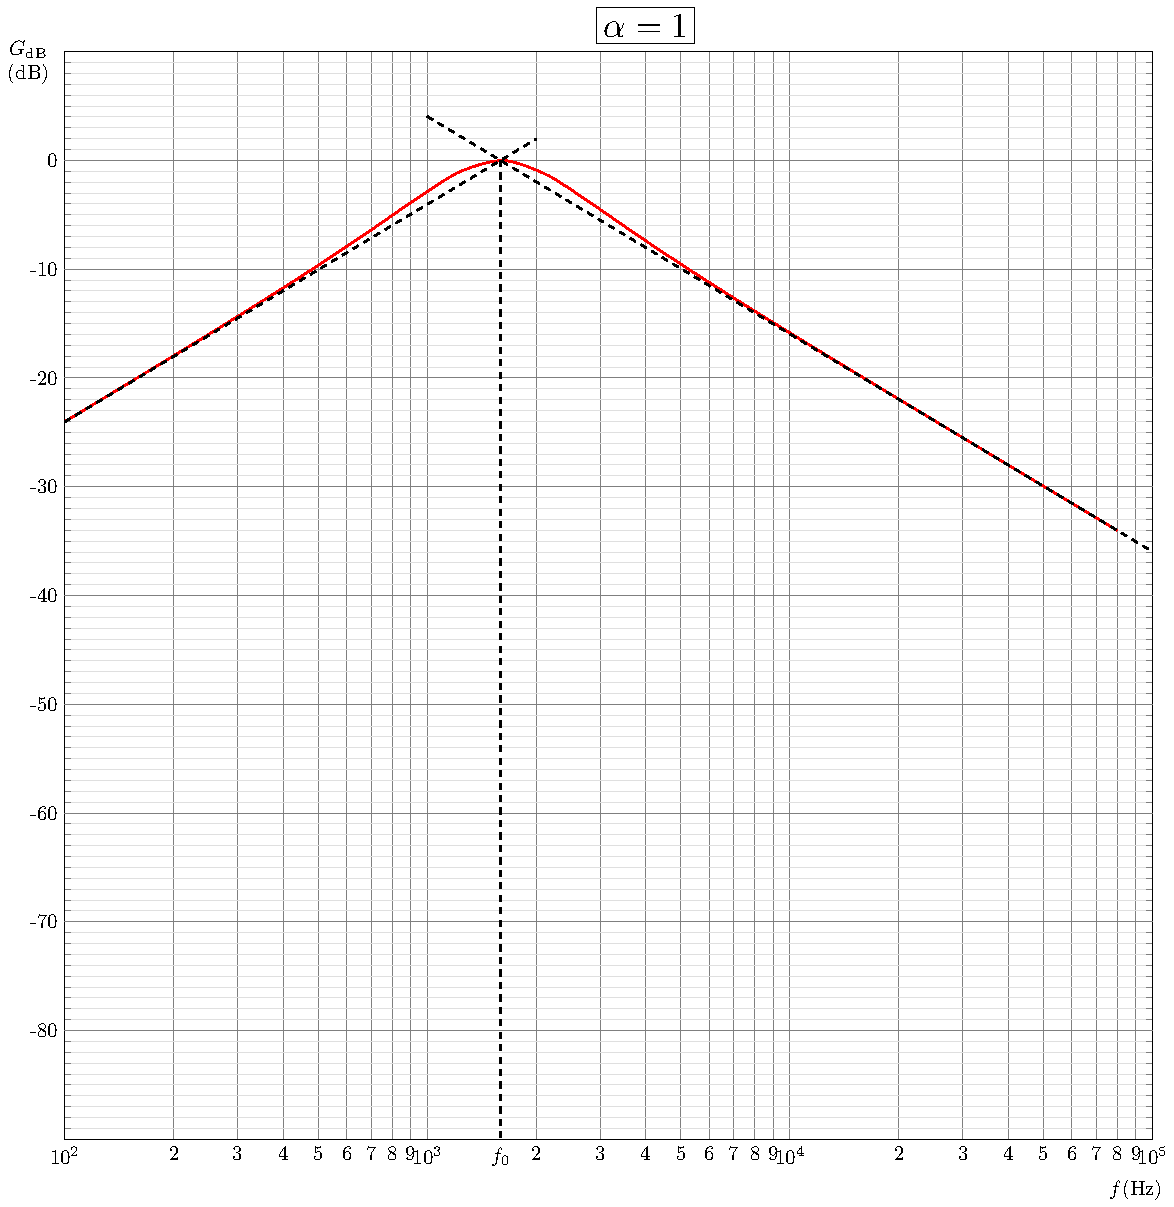
\includepdf{semilog_a1}
}{
	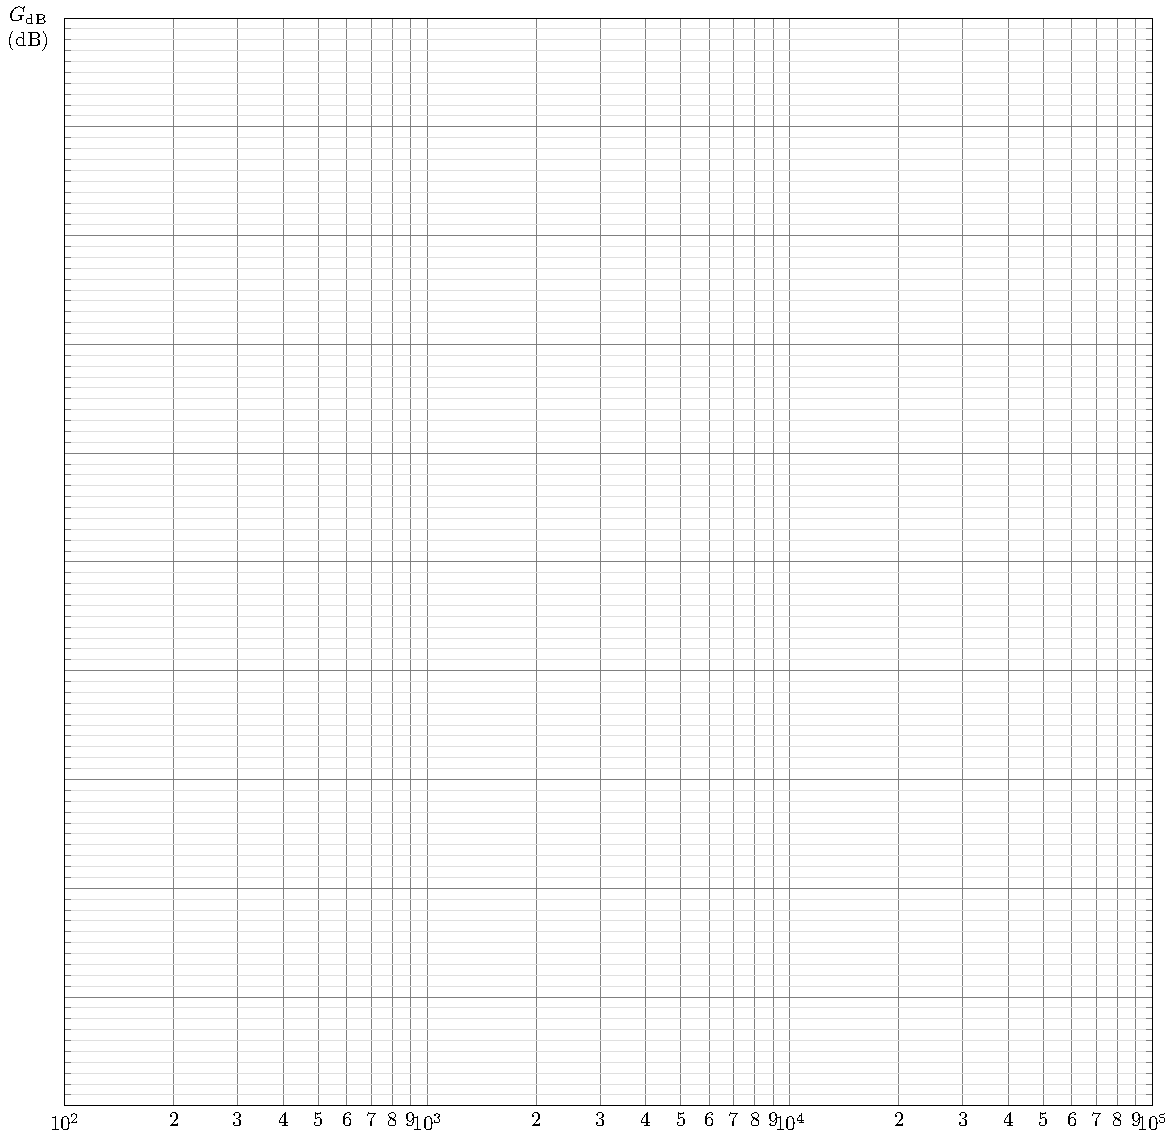
\includepdf{semilog}
}

\let\clearpage\relax

\newpage

\thispagestyle{empty}
\cswitch{
	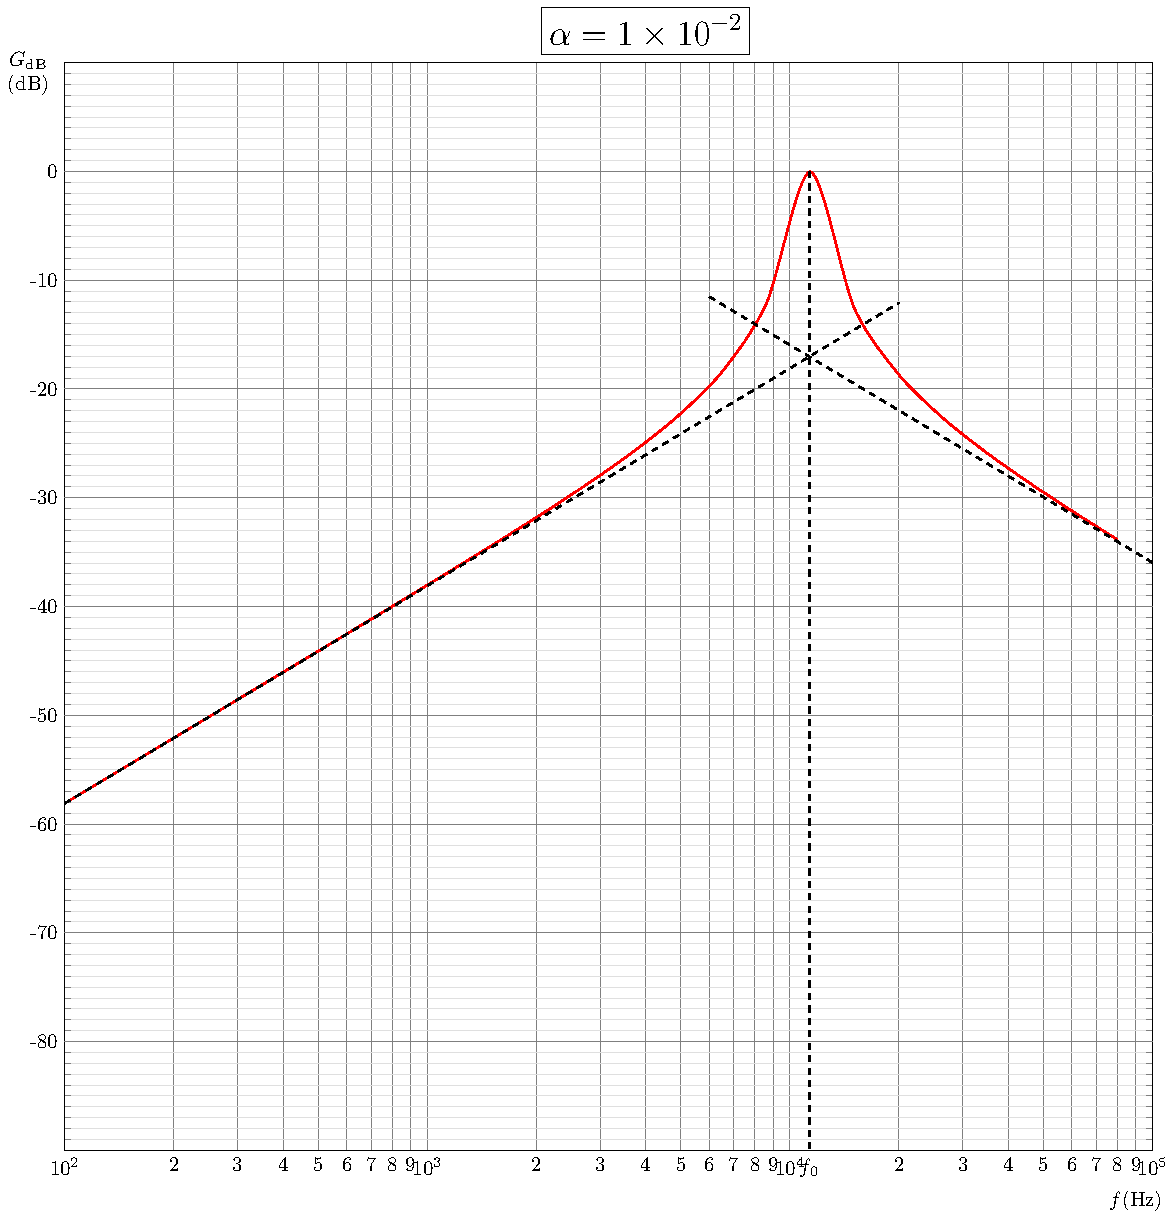
\includepdf{semilog_a1e2}
}{
	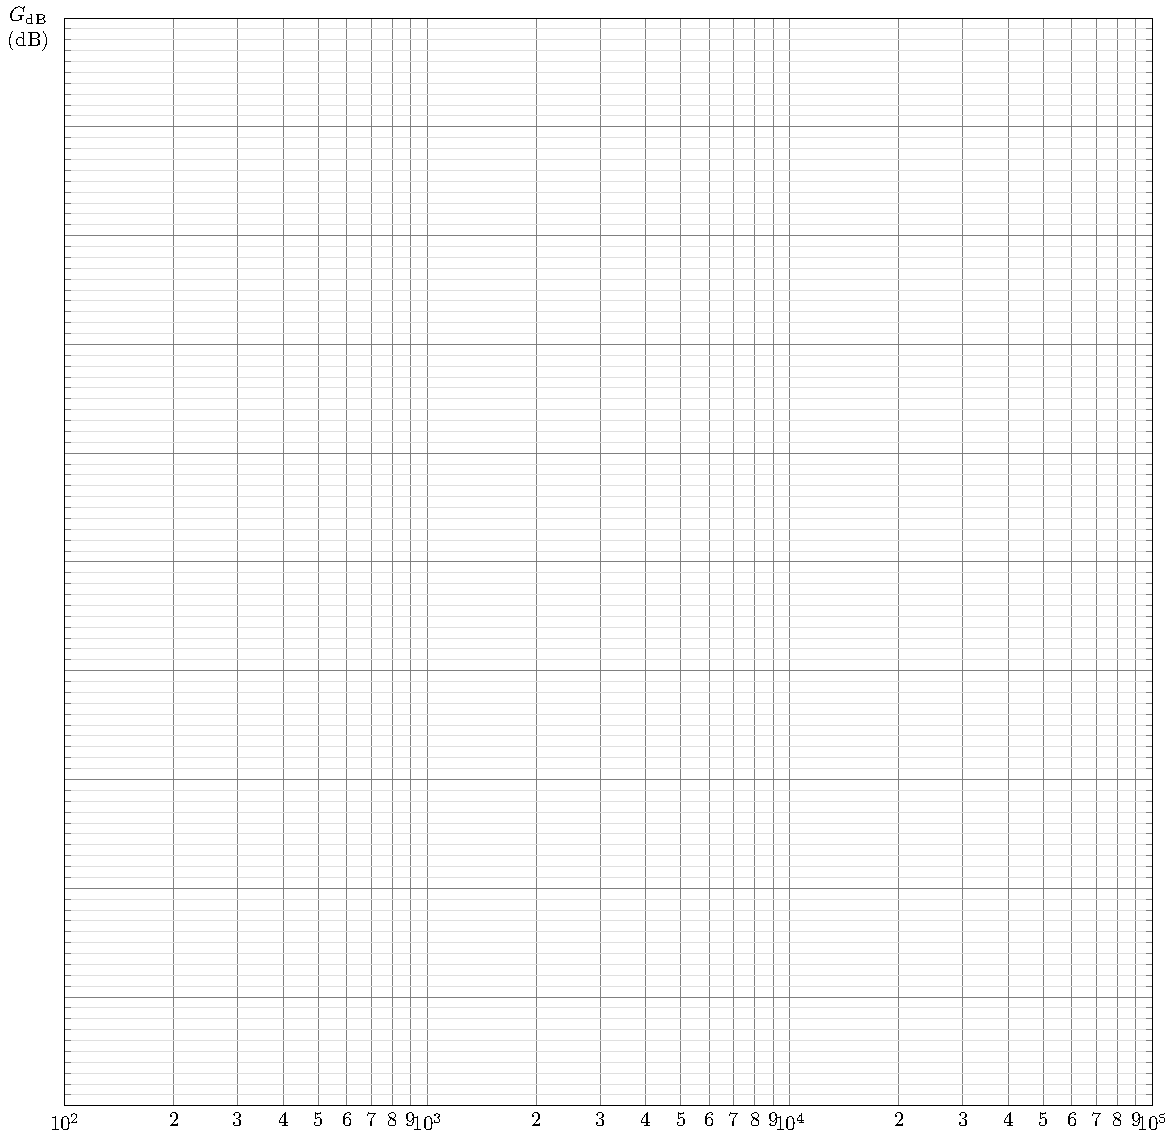
\includepdf{semilog}
}

\let\clearpage\relax
\end{document}
